\documentclass[acmtog]{acmart}
\usepackage{lipsum}
\usepackage{physics}

\usepackage{caption}
\usepackage{subcaption}

% \usepackage{titlesec}
\usepackage{graphicx}
\usepackage{xcolor}

\newcommand{\draft}[1]{\noindent\textcolor{red}{#1}}
\newcommand{\ddotproduct}[2]{#1 \hspace{-1pt}:\hspace{-1pt} #2}
\newcommand{\nfrac}[2]{#1/#2}

\setcopyright{none} 
\makeatletter
\let\@authorsaddresses\@empty\makeatother
\settopmatter{printacmref=false}
\renewcommand\footnotetextcopyrightpermission[1]{}
\AtBeginDocument{%
  \providecommand\BibTeX{{%
    Bib\TeX}}}
\begin{document}

\title{CompSim hand-in week 6/7}
\author{Carl Ivarsen Askehave}
\affiliation{
  \institution{(wfq585)}
  \country{University of Copenhagen}
}

\maketitle
\thispagestyle{empty}
\section*{The finite volume method}
\subsection*{Difference between FEM, FVM and FDM}
The finite element method (FEM), finite volume method (FVM) and finite difference method (FDM) are all methods for numerically solving PDEs. The main difference between the three methods is how they approximate the solution over the domain. The FEM approximates the solution by a sum of values weighted by carefully chosen shape functions. The FDM approximates the PDE by differences in the function values between the finitely seperated grid points of the domain.

The FVM approximates the solution to the PDE by integrating the midpoint approximation of the PDE over piecewise continuous surfaces of a number of control volumes that comprise the whole domain. The idea behind the method is, to approximate the integral form of the PDE by using the divergence theorem and the conservation laws adhering to this to convert volume integrals into surface integrals, and then approximating these using the midpoint approximation to evaluate these.

The method is conservative, and it is used in many areas of computational physics, including fluid dynamics, heat transfer, and electromagnetism, as we'll se in the following sections. Firstly we'll lay out the essential steps in the FVM, and then we'll apply it to a few different problems.

\section{The steps of the FVM}
\begin{enumerate}
  \item[\textbf{Step 1:}] \textbf{Governing equation.} Start with a PDE that describes the physical problem.
  \item[\textbf{Step 2:}] \textbf{Mesh layout.} Divide the domain into a number of control volumes.
  \item[\textbf{Step 3:}] \textbf{Volume integral.} Given a PDE, integrate it over the domain.
  \item[\textbf{Step 4:}] \textbf{Use Gauss' divergence theorem.} Rewrite the relevant parts into surface integrals.
  \item[\textbf{Step 5:}] \textbf{Piecewise continuous integrals.} Divide the surface integral into piecewise continuous integrals. This step is very dependent on the mesh layout that you choose to use.
  \item[\textbf{Step 6:}] \textbf{Time derivative.} If the PDE has a time derivative, use Leibniz's rule to pull the it outside the volume integral.
  \item[\textbf{Step 7:}] \textbf{Numerical integration.} Approximate the surface integrals of the directional derivatives by using the midpoint approximation.
  \item[\textbf{Step 8:}] \textbf{Boundary conditions.} Apply the boundary conditions specific to the problem.
  \item[\textbf{Step 9:}] \textbf{Assemble the linear system.} Assemble the equations into a linear system.
  \item[\textbf{Step 10:}] \textbf{Time discretization.} Discretize the time derivative using any relevant time integration scheme.
  \item[\textbf{Step 11:}] \textbf{Compute the solution.} Compute the solution.
\end{enumerate}
% \subsection*{Step 1: Volume integral}
% We take the integral of the PDE over the volume of the domain
% %
% \begin{equation}
%   \int_V \qty(\frac{\partial g(\boldsymbol x)}{\partial t} + \boldsymbol \nabla \cdot \boldsymbol f (\boldsymbol x)) \, dV = \int_V 0 \, dV.
% \end{equation}
% \begin{equation}
%   \int_V \frac{\partial g(\boldsymbol x)}{\partial t} \, dV = - \int_V \boldsymbol \nabla \cdot \boldsymbol f (\boldsymbol x) \, dV. \label{eq:volint}
% \end{equation}
% %

% \subsection*{Step 2: Use Gauss' divergence theorem}
% \textit{Gauss' divergence theorem} states that for a vector field $\boldsymbol f$ and a domain $\Omega$ with volume $V$ and surface $S$, we have
% %
% \begin{equation}
%   \int_V \boldsymbol \nabla \cdot \boldsymbol f \, dV = \oint_S \boldsymbol f \cdot \boldsymbol n \, dS,
% \end{equation}
% %
% where $\boldsymbol n$ is the outward unit normal to the surface $S$. This means that we can rewrite the volume integral in (\ref{eq:volint}) as a surface integral, leaving us with
% %
% \begin{equation}
%   \int_V \frac{\partial g(\boldsymbol x)}{\partial t} \, dV = - \oint_S \boldsymbol f (\boldsymbol x) \cdot \boldsymbol n \, dS. \label{eq:surfint}
% \end{equation}
% %

\section{Conservation of the integral form}
Suppose we have a PDE
%
\begin{equation}
  \frac{\partial g(\boldsymbol x)}{\partial t} + \boldsymbol \nabla \cdot \boldsymbol f (\boldsymbol x) = 0, \label{eq:pde}
\end{equation}
%
where $g$ is some scalar function of the vector field $\boldsymbol x$, and $\boldsymbol f$ is a vector function of $\boldsymbol x$.
Suppose now that we're interested in calculating this over a domain $\Omega$ which is divided into two parts $\Omega_A$ and $\Omega_B$ with total boundary $\partial \Omega = \partial \Omega_A + \partial \Omega_B$ as shown in Figure\ \ref{fig:vol2}. In the process we created a new surface region that the two domains share, and the respective surfaces of the two new volumes then become the union of their respective parts of the old surface $S_a$ and $S_a$ and their new shared interface $S_c$ as such
%
\begin{align}
  S_A = S_a \cup S_c, \quad \text{and} \quad S_B = S_b \cup S_c.
\end{align}
%
\begin{figure}
  \centering
  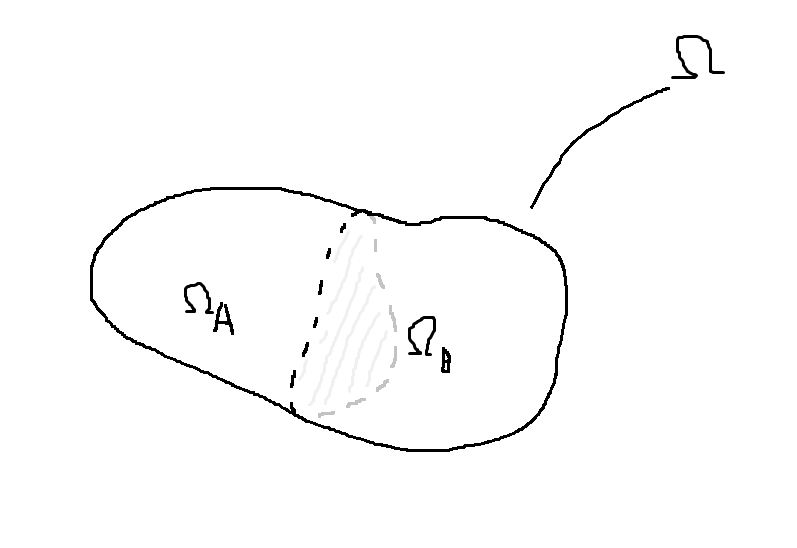
\includegraphics[width=0.4\textwidth]{Images/volume2.png}
  \caption[Toy domain split]{The domain $\Omega$ split into two subdomains $\Omega_A$ and $\Omega_A$.\label{fig:vol2}}
\end{figure}
%
This allows us to rewrite the surface integral as a sum of the integrals over the two new surfaces
\begin{multline}
  \int_{V_A} \frac{\partial g(\boldsymbol x)}{\partial t} \, dV + \int_{V_B} \frac{\partial g(\boldsymbol x)}{\partial t} \, dV\\
  = - \oint_{S_a} \boldsymbol f (\boldsymbol x) \cdot \boldsymbol n_a \, dS - \oint_{S_c} \boldsymbol f (\boldsymbol x) \cdot \boldsymbol n_c \, dS\\
  - \oint_{S_b} \boldsymbol f (\boldsymbol x) \cdot \boldsymbol n_b \, dS - \oint_{S_c} \boldsymbol f (\boldsymbol x) \cdot (- \boldsymbol n_c) \, dS,
\end{multline}
%
where we've used the fact that the normal vector $\boldsymbol n_c$ points in the opposite direction deppending on which volume we're integrating over. This means that the surface integrals over the shared interface $S_c$ cancel out, and we're left with
%
\begin{multline}
  \int_{V_A} \frac{\partial g(\boldsymbol x)}{\partial t} \, dV + \int_{V_B} \frac{\partial g(\boldsymbol x)}{\partial t} \, dV\\
  = - \oint_{S_a} \boldsymbol f (\boldsymbol x) \cdot \boldsymbol n_a \, dS - \oint_{S_b} \boldsymbol f (\boldsymbol x) \cdot \boldsymbol n_b \, dS,
\end{multline}
%
but since $V_A \cup V_B = V$ and $S_a \cup S_b = S$, this is equivalent to
%
\begin{equation}
  \int_V \frac{\partial g(\boldsymbol x)}{\partial t} \, dV = - \oint_{S} \boldsymbol f (\boldsymbol x) \cdot \boldsymbol n \, dS,
\end{equation}
%
which is exactly the volume integral of (\ref{eq:pde}). This showcases that, when using the divergence theorem, the integral form of the PDE is conserved regardless of how many times we subdivide the domain, as long as the boundaries of the subdivision are piecewise continuous.

% \subsection*{Step 3: Piecewise continuous integrals}
% We divide the surface integral into a number of integrals over piecewise continuous surfaces $S_e$, summing over them all
% %
% \begin{equation}
%   \int_V \frac{\partial g(\boldsymbol x)}{\partial t} \, dV = - \sum_e \oint_{S_e} \boldsymbol f (\boldsymbol x) \cdot \boldsymbol n_e \, dS.
% \end{equation}

% \subsection*{Step 4: Time derivative}
% If we have a time derivative inside the volume integral, we can use Leibniz's rule to pull it outside the integral
% %
% \begin{equation}
%  \frac{\partial}{\partial t} \int_V g(\boldsymbol x) \, dV = - \sum_e \oint_{S_e} \boldsymbol f (\boldsymbol x) \cdot \boldsymbol n_e \, dS,
% \end{equation}
% %
% the proof of which we'll skip here.

% \subsection*{Step 5: Numerical integration}
% The method of integration chosen here, can differ depending on what mesh layout we've chosen. In our case, we look at the control volume $c$ in our mesh, and approximate the function $\boldsymbol f$ by evaluating it in the midpoint $\boldsymbol x_m = (\boldsymbol x_c + \boldsymbol x_e) / 2$ between the two control volumes $c$ and $e$
% %
% \begin{equation}
%   \boldsymbol f (\boldsymbol x) \approx \boldsymbol f (\boldsymbol x_m).
% \end{equation}
% %
% Thus our integrals become
% %
% \begin{equation}
%   \sum_e \oint_{S_e} \boldsymbol f (\boldsymbol x) \cdot \boldsymbol n_e \, dS \approx \sum_e \boldsymbol f (\boldsymbol x_e) - \boldsymbol f (\boldsymbol x_c) \frac{A_e}{s_{ce}},
% \end{equation}
% %
% where we've defined $s_{ce} = \lVert \boldsymbol x_e - \boldsymbol x _c \rVert$ and $A_e$ is the area of the shared surface between $c$ and $e$. This equation holds for all the control volumes, and writing it out for a single control volume $c$ with $N$ neighbouring control volumes $e \in (0,1,\dots, N) \, ; \ e \neq c$ and $\boldsymbol f_{ce} = \boldsymbol f\left(\nfrac{\boldsymbol x_c + \boldsymbol x_e}{2}\right)$ gives
% %
% \begin{multline}
%   (\boldsymbol x_0 - \boldsymbol x_c) \frac{l_0}{s_{c0}} + (\boldsymbol x_1 - \boldsymbol x_c) \frac{l_1}{s_{c1}} + \cdots + (\boldsymbol x_N - \boldsymbol x_c) \frac{l_N}{s_{cN}}\\
%   = \boldsymbol f_{c0} \cdot \boldsymbol n_0 l_0 + \boldsymbol f_{c1} \cdot \boldsymbol n_1 l_1 + \cdots + \boldsymbol f_{cN} \cdot \boldsymbol n_N l_N.
% \end{multline}
% %

\section{2D magnetostatic problem}
\subsection*{Step 1: Governing equation}
Magnetization is explicitly governed by the relations
%
\begin{equation}
  \boldsymbol B = \mu_0 \left(\boldsymbol M + \boldsymbol H\right) \quad \text{and} \quad \nabla \times \boldsymbol H = \boldsymbol 0,
\end{equation}
%
the latter of which has the general solution $\boldsymbol H = - \nabla \phi$ where $\phi$ is a scalar potential field, which means that the first equation can be rewritten as
%
\begin{equation}
  \boldsymbol B = \mu_0 \left(\boldsymbol M - \nabla \phi \right)
\end{equation}
%
and then taking the divergence of both sides gives
%
\begin{equation}
  \nabla \cdot \boldsymbol B = \mu_0 \left( \nabla \cdot \boldsymbol M - \nabla \cdot \nabla \phi \right) = 0.
\end{equation}
%
Cleaning up we obtain
%
\begin{equation}
  \nabla \cdot \nabla \phi = \nabla \cdot \boldsymbol M
\end{equation}
%
This is a Poisson equation to solve for $\phi$, and will be our governing equation. It is defined on a closed 2d box with dimensions $[-3, 3] \times [-1, 1]$, and for the magnetization $\boldsymbol M$ we have
%
\begin{equation}
  \boldsymbol M = \begin{pmatrix}
    0 \\ -1
  \end{pmatrix} \quad \text{inside the unit circle}.
\end{equation}
%
Along with these we enforce the north pole boundary condition
%
\begin{equation}
  \phi = 0 \quad \text{for} \quad \boldsymbol x = \boldsymbol x_{NP},
\end{equation}
%
where $\boldsymbol x_{NP}$ is the position of the vertex closest to the north pole of the magnet. At every other point we have von Neumann or no-flux boundary conditions
%
\begin{equation}
  \boldsymbol \nabla \phi \cdot \boldsymbol n = 0, \quad \text{for} \quad \boldsymbol x \in \partial \Omega.
\end{equation}
%


\subsection*{Step 2: Mesh layout}
To divide the domain into control volumes, we'll start with a triangular mesh, and construct the control volumes around each vertex in the mesh as shown in Figure\ \ref{fig:cv1}. We see that the control volumes for the vertices on the boundary differing shapes from the interior vertices. We will have to take this into account when we derive the method.

\begin{figure}
  \centering
  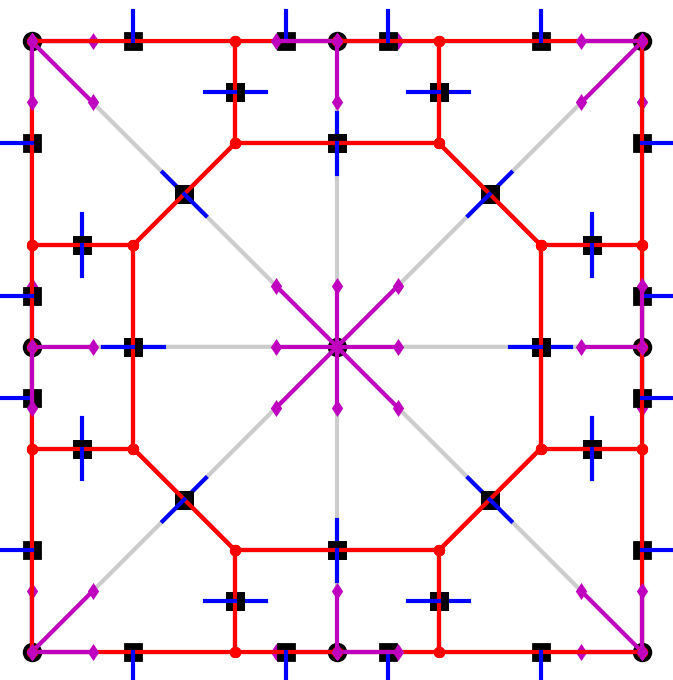
\includegraphics[width=0.25\textwidth]{Images/cv1.png}
  \caption{Debugging view of a section of our triangular mesh with one control volume corresponding to the middle vertex. The surface elements of the control volume consists of piecewise linear segments connecting the central nodes of each triangle with the midpoints on their sides going in a counterclockwise fashion around the control volume vertex.\label{fig:cv1}}
\end{figure}

\subsection*{Step 3: Volume integral}
We integrate on both sides
%
\begin{align}
  \int_V \boldsymbol \nabla \cdot \boldsymbol \nabla \phi \, dV = \int_V \boldsymbol \nabla \cdot \boldsymbol M \, dV
\end{align}
%

\subsection*{Step 4: Use gauss' divergence theorem}
%
\begin{equation}
  \oint_S \boldsymbol \nabla \phi \cdot \boldsymbol n  \, d S = \oint_S \boldsymbol M \cdot \boldsymbol n \, d S
\end{equation}
%

\subsection*{Step 5: Piecewise continuous integrals}
%
\begin{equation}
  \sum_e \int_{S_e} \boldsymbol \nabla \phi \cdot \boldsymbol n_e \, d S = \sum_e \int_{S_e} \boldsymbol M \cdot \boldsymbol n_e \, d S
\end{equation}
%

\subsection*{Step 6: Time derivative}
We don't have a time derivative in this case, but if we did, we'd use Leibniz's rule to pull the time derivative outside the volume integral
%
\begin{equation}
  \int_V \frac{ \partial f }{ \partial t }  \, dV = \frac{ \partial  }{ \partial t} \int_V f \, dV
\end{equation}
%

\subsection*{Step 7: Numerical integration}
We approximate the directional derivative $\boldsymbol \nabla\phi \cdot \boldsymbol n$ at the midpoint $\boldsymbol x_m = (\boldsymbol x_c + \boldsymbol x_e) / 2$, by using the FDM:\@
%
\begin{equation}
  \boldsymbol \nabla \phi \cdot \boldsymbol n_e \approx \frac{\phi(\boldsymbol x_e) - \phi(\boldsymbol x_c)}{\lVert \boldsymbol x_e  - \boldsymbol x_c \rVert}.
\end{equation}
%
Since the integrals are over piecewise linear segments, we get:
%
\begin{equation}
  \sum_e \phi(\boldsymbol x_e) - \phi(\boldsymbol x_c) \frac{l_e}{s_{ce}  } = \sum_e \boldsymbol M\left( \frac{\boldsymbol x_c + \boldsymbol x_e}{2} \right) \cdot \boldsymbol n_e l_e \label{eq:num_int1}
\end{equation}
%
where we've defined $s_{ce} = \lVert \boldsymbol x_e - \boldsymbol x _c \rVert$.

\subsection*{Step 8: Boundary conditions}
We have the north pole boundary condition $\phi = 0$ at the north pole vertex, and the von Neumann boundary conditions $\boldsymbol \nabla \phi \cdot \boldsymbol n = 0$ at all other vertices. And since
%
\begin{equation}
  \oint_{S} \boldsymbol \nabla \phi \cdot \boldsymbol n \, dS = \oint_{S} \boldsymbol 0 \, dS = 0
\end{equation}
%
at the boundary.

\subsection*{Step 9: Assemble the linear system}
Equation (\ref{eq:num_int1}) holds for each control volume, and writing it out for a single control volume $c$ with $N$ neighbouring control volumes $e \in (0,1,\dots, N) \, ; \ e \neq c$ and $\boldsymbol M_{ce} = \boldsymbol M\left(\nfrac{\boldsymbol x_c + \boldsymbol x_e}{2}\right)$ gives
%
\begin{multline}
  (\phi_0 - \phi_c) \frac{l_0}{s_{c0}} + (\phi_1 - \phi_c) \frac{l_1}{s_{c1}} + \cdots + (\phi_N - \phi_c) \frac{l_N}{s_{cN}}\\
  = \boldsymbol M_{c0} \cdot \boldsymbol n_0 l_0 + \boldsymbol M_{c1} \cdot \boldsymbol n_1 l_1 + \cdots + \boldsymbol M_{cN} \cdot \boldsymbol n_N l_N
\end{multline}
%
We're trying to assemble the equation into a linear system $\boldsymbol A \boldsymbol y = \boldsymbol b$, with $\boldsymbol A$ being $(N \times N)$ and $\boldsymbol b$ being $(N \times 1)$, where $N$ is the total number of control volumes. This means that we end up with $N$ equations on the form
%
\begin{equation}
  A_{i0} \, y_0 + \cdots + A_{i N} \, y_N= b_i
\end{equation}
%
This way, if we let $y_e = \phi_e$ and furthermore
%
\begin{equation}
  A_{ce} = \frac{l_e}{s_{ce}}, \quad A_{cc} = - \sum_e \frac{l_e}{s_{ce}} \quad \text{and} \quad b_c = \sum_e \boldsymbol M_{ce} \cdot \boldsymbol n_e l_e
\end{equation}
%
our linear system $\boldsymbol A \boldsymbol y = \boldsymbol b$ should be equivalent to our discretized relation above. For the von Neumann boundary conditions, we just set $A_{ce} = 0$, $A_{cc} = 0$ and $b_c = 0$ for the boundary vertices.
%

Since we have no time dependence in this problem, we can solve the linear system directly, which gives us the solution to the magnetostatic problem, meaning that we skip the last steps of the FVM.\@

The solution to the problem is shown in Figure\ \ref{fig:mag_sol1}, where we see the scalar potential field $\phi$ in the domain. We see that the potential is zero at the north pole, and that the potential is higher at the south pole, which is what we would expect from a magnetostatic problem.

\begin{figure}
  \centering
  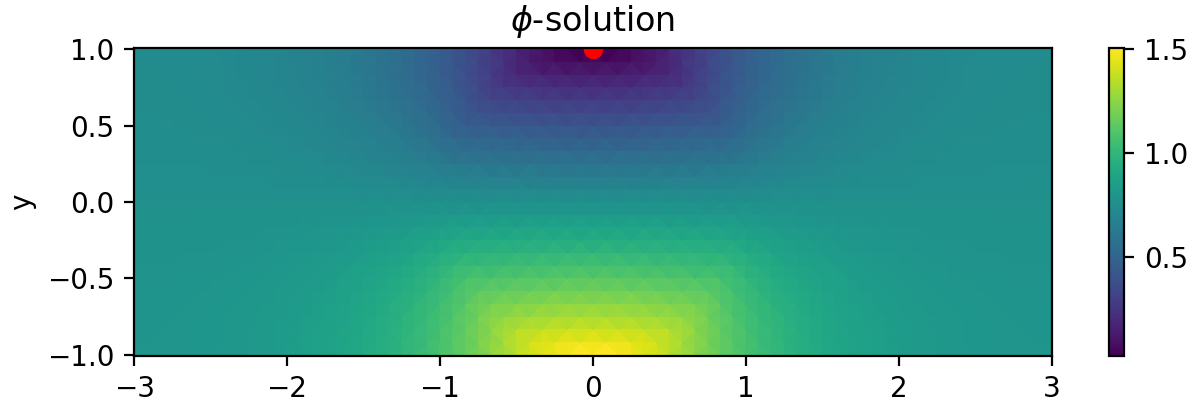
\includegraphics[width=0.47\textwidth]{Images/mag_sol1.png}
  \caption{The solution to the magnetostatic problem. The scalar potential field $\phi$ is shown in the domain, with the north pole at the top indicated by the red dot.\label{fig:mag_sol1}}
\end{figure}

\begin{figure}
  \centering
  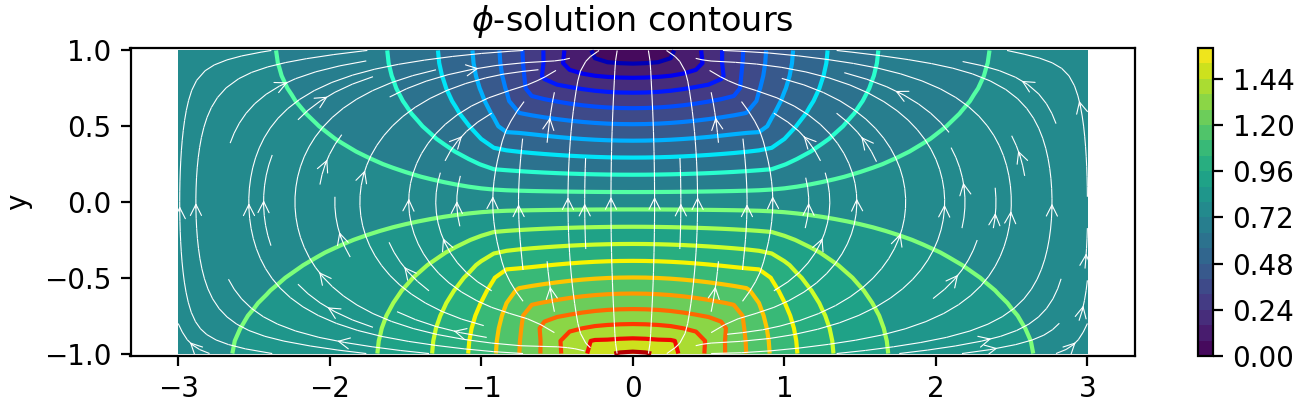
\includegraphics[width=0.47\textwidth]{Images/field_lines.png}
  \caption{Here is seen the solution from \ref{fig:mag_sol1}, with magnetic field streamlines (white arrows) and contours(colorful lines).\label{fig:field_lines}}
\end{figure}

\begin{figure}
  \centering
  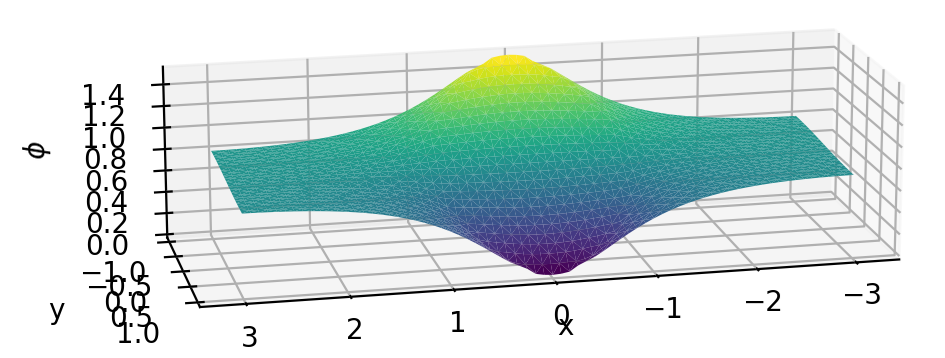
\includegraphics[width=0.47\textwidth]{Images/mag_sol1_3d.png}
  \caption{A 3d perspective on Fig. \ref{fig:mag_sol1}.\label{fig:mag_sol1_3d}}
\end{figure}



\section{Dynamic 2D hyperelastic problem}
\subsection*{Step 1: Governing equation}

The physics of hyperelastic materials are described by the Cauchy equation, here given wrt.\ the material coordinates $\boldsymbol X$ (although $\ddot{\boldsymbol x}$ still refers to the spatial acceleration):
%
\begin{equation}
  \rho_0 \ddot{\boldsymbol x} = \boldsymbol b_0 + \boldsymbol \nabla_{\boldsymbol X} \cdot \boldsymbol P, \label{eq:cauchy}
\end{equation}
%
where $\rho_0$ is the material density, $\boldsymbol b_0$ is the body force per unit volume acting on the material and $\boldsymbol P$ is the first Piola–Kirchhoff stress tensor. Applying a traction force to part of the boundary $\Gamma_T$, Cauchy's stress hypothesis gives
%
\begin{equation}
  \boldsymbol P \boldsymbol N = \boldsymbol t \quad \text{for} \quad \boldsymbol x \in \Gamma_T,
\end{equation}
%
where $\boldsymbol N$ is the unit outward normal, and $\boldsymbol t$ is the traction force. We also have the constitutive equation in the form of the isotropic, hyperelastic Saint-Venant-Kirchhoff law:
%
\begin{equation}
  \boldsymbol S = \lambda \,\mathrm{tr}(\boldsymbol E) \boldsymbol I + 2 \mu \boldsymbol E
\end{equation}
%
where $\boldsymbol E$ is the Lagrangian Green strain given by
%
\begin{equation}
  \boldsymbol E = \frac{1}{2} \left[ {(\boldsymbol \nabla_{\boldsymbol X} \boldsymbol u)}^T + \boldsymbol \nabla _{\boldsymbol X} \boldsymbol u + {(\boldsymbol \nabla _{\boldsymbol X} \boldsymbol u)}^T \cdot \boldsymbol \nabla _{\boldsymbol X} \boldsymbol u \right]  = \frac{1}{2} (\boldsymbol F^T \boldsymbol F - \boldsymbol I),
\end{equation}
%
where $\boldsymbol F$ is the deformation gradient. The second Piola–Kirchhoff stress tensor  $\boldsymbol S$ is related to the first by
%
\begin{equation}
  \boldsymbol P = \boldsymbol F \boldsymbol S.
\end{equation}
%
\subsection*{Step 2: Mesh layout}
We use the median-dual-centered-vertex-control-volume which is a mesh layout that is well-suited for the FVM, and will give us the power to make a smart re-writing later on in the process. The mesh layout is shown in Figure\ \ref{fig:mesh1}.

\begin{figure}
  \centering
  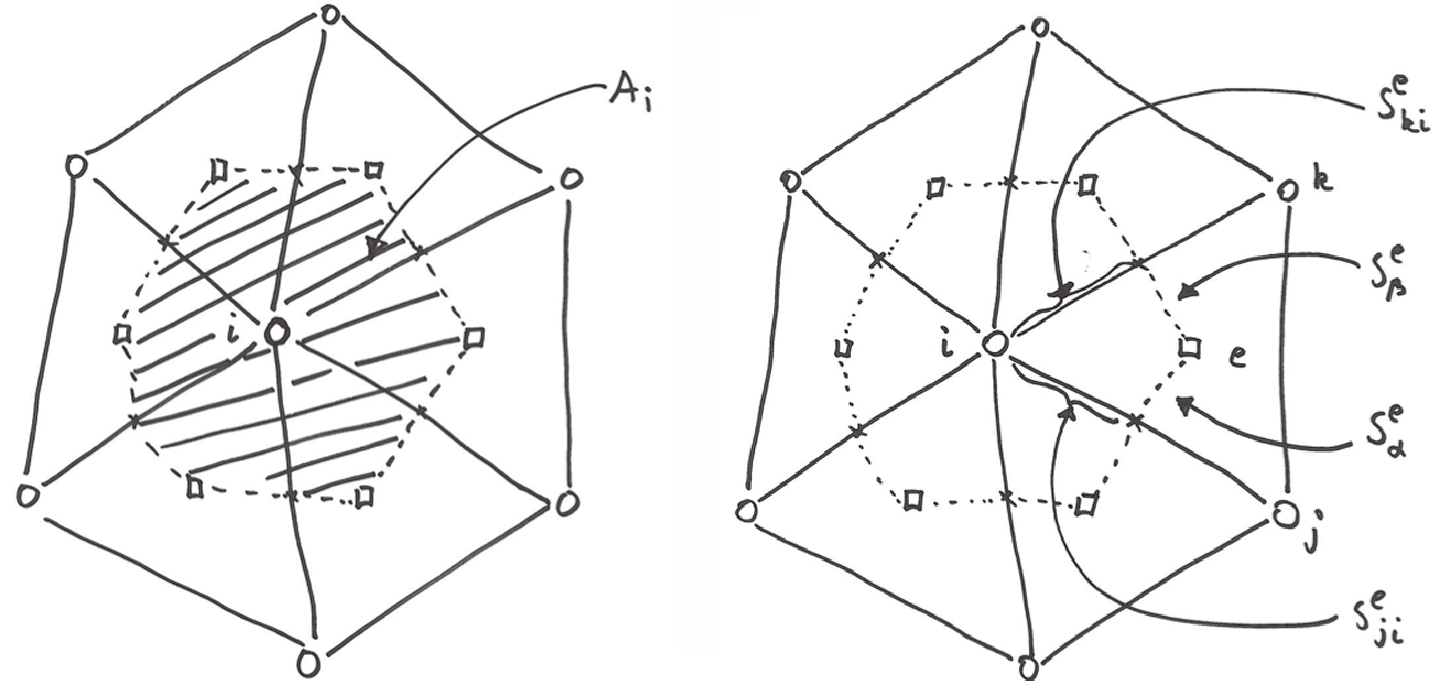
\includegraphics[width=0.47\textwidth]{Images/cv2.png}
  \caption{An interior cell of median-dual-centered-vertex-control-volume mesh layout. The control volume is centered around the vertex $i$, and the surface elements are piecewise linear segments connecting the central nodes of each triangle with the midpoints on their sides going in a counterclockwise fashion around the control volume vertex. The names for the sides corresponding to the neighbouring element $e$ are $S^e_{ij}$, $S^e_{\alpha}$, $S^e_{\beta}$ and $S^e_{ki}$.\label{fig:mesh1}}
\end{figure}

\subsection*{Step 3: Volume integral}
We integrate (\ref{eq:cauchy}) over the $i$'th control volume
%
\begin{equation}
  \int_{V_i} \rho_0 \frac{ \partial^{2} \boldsymbol x }{ \partial t^{2} }  \, d V = \int_{V_i} \boldsymbol b_0 \, d V + \int_{V_i} \boldsymbol \nabla_{\boldsymbol X} \cdot \boldsymbol P \, d V
\end{equation}


\subsection*{Step 4: Use Gauss' divergence theorem}
Assuming that the external force $\boldsymbol b_0$ is constant over the control volume, and using Gauss' divergence theorem and Leibniz' rule, we get
%
\begin{equation}
  \frac{ \partial^{2} }{ \partial t^{2} } \int_{V_i} \rho_0 \boldsymbol x \, d V = V_i\boldsymbol b_{0i} + \oint_{S_i} \boldsymbol P \boldsymbol N \, dS.
\end{equation}
%
Assuming that the material density $\rho_0$ is also constant, we get
%
\begin{equation}
  m_i \frac{ \partial^{2} }{ \partial t^{2} } \left(\boldsymbol x_i \right)  = V_i \boldsymbol b_{0i} + \oint_{S_i} \boldsymbol P \boldsymbol N \, dS,
\end{equation}
%
where $\boldsymbol x_i$ is the center of the $i$'th control volume.


\subsection*{Step 5: Piecewise continuous integrals}
Now we use the fact that each segment of the boundary is piecewise continuous to get:
%
\begin{equation}
  m_i \ddot{\boldsymbol x}_i = V_i \boldsymbol b_{0i} + \sum_e \sum_\gamma \oint_{S_\gamma^e}\boldsymbol P \boldsymbol N \, dS
\end{equation}
%
The edge segments are each uniquely identified by the triangle neighbouring their control volume $e$, and the part of the index of segments lying inside that triangle $\gamma \in (\alpha, \beta)$.

To deduce the value of the integral we start by looking at the three types of edges in the mesh. The first type is the edges lying on the boundary of the domain where no traction force is applied. Here $\boldsymbol P \boldsymbol N = \boldsymbol t = \boldsymbol 0$, and so their integrals are also zero, so we disregard these.

The second type is the edges lying on the boundary of the domain where the traction force IS applied. Here $\boldsymbol P \boldsymbol N = \boldsymbol t$, which is constant, and thus the integrals here become
%
\begin{equation}
  \oint_{S_\gamma^e} \boldsymbol t \, dS = \boldsymbol t \,l_\gamma^e
\end{equation}
%
The third type consists of the edges inside the domain, where we'll use the midpoint approximation to get (for the $\alpha$'th segment of the control volume edge)
%
\begin{equation}
  \oint_{S_\gamma^e} \boldsymbol P \boldsymbol N \, dS \approx \boldsymbol P(\boldsymbol x_\gamma^e) \boldsymbol N_\gamma^e \, l_\gamma^e \ ,
\end{equation}
%
where $\boldsymbol x_\gamma^e$ is the centerpoint of the segment. This means that our equation becomes
%
\begin{align}
  m_i \ddot{\boldsymbol x}_i & = V_i \boldsymbol b_{0i} +  \sum_e \sum_\gamma \boldsymbol t \, l_\gamma^e + \sum_e \boldsymbol P(\boldsymbol x_\gamma^e) \boldsymbol N_\gamma^e \\
  m_i \ddot{\boldsymbol x}_i & = \boldsymbol f_{\mathrm{ext}, i} + \boldsymbol f_{t,i} + \boldsymbol f_{\mathrm{ela},i}
\end{align}
%
So here we have an equation that describes the total force acting on the $i$'th control volume, where $\boldsymbol f_{\mathrm{ext},i}$ denotes the external forces, $\boldsymbol f_{t,i}$ denotes the traction forces, and $\boldsymbol f_{\mathrm{ela},i}$ denotes the elastic forces.

\subsubsection*{Computing the deformation gradient}
We glossed over one thing though, and that is computing the midpoint rule approximation of the integral over the stress tensor $\boldsymbol P(\boldsymbol x_\alpha^e) \boldsymbol N_\alpha^e \, l_\gamma^e$. We know both $\boldsymbol N_\alpha^e$ and $l_\gamma^e$ so we'll focus on the last part. We know that
%
\begin{equation}
  \boldsymbol P(\boldsymbol x) = \boldsymbol F(\boldsymbol x) \boldsymbol S, \quad \boldsymbol S = \lambda \,\mathrm{tr}(\boldsymbol E) \boldsymbol I + 2 \mu \boldsymbol E, \quad \mathrm{and} \quad \boldsymbol E = \frac{1}{2} (\boldsymbol F^T \boldsymbol F - \boldsymbol I),
\end{equation}
%
and so we need to compute the deformation gradient $\boldsymbol F$. We start by introducing a deformation field $\phi$ that maps the material coordinates $\boldsymbol X$ into the spatial coordinates $\boldsymbol x$, as such $\boldsymbol x = \phi(\boldsymbol X)$. Now the deformation gradient is defined as
%
\begin{equation}
  \boldsymbol F = \frac{ \partial \boldsymbol x }{ \partial \boldsymbol X } = \frac{ \partial \phi(\boldsymbol X) }{ \partial \boldsymbol X }, \qquad \implies \qquad d\boldsymbol x = \boldsymbol F \, d\boldsymbol X.
\end{equation}
%

\begin{figure}
  \centering
  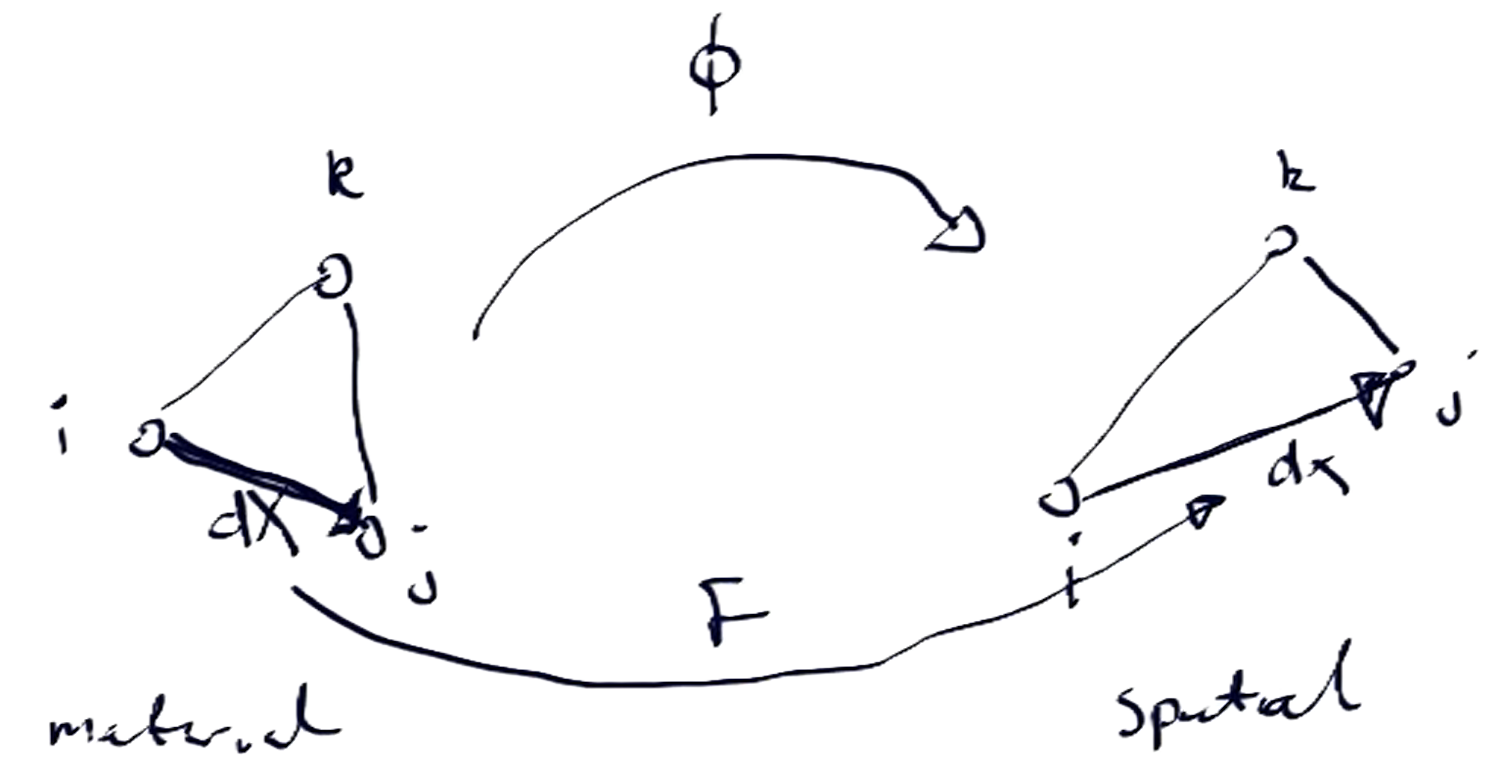
\includegraphics[width=0.4\textwidth]{Images/deform_field.png}
  \caption{An example of the same triangle element before and after applying the deformation field $\phi$. The $d \boldsymbol X$ vector becomes $\boldsymbol F \, d\boldsymbol X = d d\boldsymbol x $.\label{fig:deform_field}}
\end{figure}


Assuming that the deformation gradient is constant over each element, $\boldsymbol F = \boldsymbol F^e$ we can use it to translate material vectors $\boldsymbol A$ and $\boldsymbol B$ into their corresponding spatial vectors $\boldsymbol a$ and $\boldsymbol b$ like this
%
\begin{equation}
  \boldsymbol D^e = \begin{bmatrix}
    a_x & b_x \\
    a_y & b_y
  \end{bmatrix} = \boldsymbol F^e \begin{bmatrix}
    A_X & B_X \\
    A_Y & B_Y
  \end{bmatrix} = \boldsymbol F^e \boldsymbol D^e_0.
\end{equation}
%
This also means that $\boldsymbol F^e = \boldsymbol D^e (\boldsymbol D_0^e)^{-1}$, and therefore (since the material coordinates are constant wrt. to time, $( \boldsymbol D_0^e )^{-1}$ can be precomputed) we just need to calculate $\boldsymbol D^e$ at each time step to get $\boldsymbol F^e$ and then use the formulas for $\boldsymbol E$, $\boldsymbol S$ and $\boldsymbol P$ to get
%
\begin{equation}
  \boldsymbol E^e = \frac{1}{2} \left( {\boldsymbol F^e}^T \boldsymbol F^e - \boldsymbol I\right) , \quad \boldsymbol S^e = \lambda \, \mathrm{tr}(\boldsymbol E^e) \boldsymbol I + 2 \mu \boldsymbol E^e, \quad \boldsymbol P^e = \boldsymbol F^e \boldsymbol S^e.
\end{equation}
%
This means that our midpoint approximation becomes
%
\begin{equation}
  \boldsymbol P(\boldsymbol x_\gamma^e) \boldsymbol N_\gamma^e \, l_\gamma^e = \boldsymbol P^e \boldsymbol N_\gamma^e \, l_\gamma^e.
\end{equation}
%
It becomes so simple, because of the fact that $\boldsymbol F$ is constant over each triangle element, and thus $\boldsymbol P^e$ ends up also being constant.

\subsubsection*{Clever rewrite of the line integral}
Using the fact that $\boldsymbol P^e$ is constant over each element and the fact that the line integral over a closed loop of a constant function is equal to zero, we can rewrite our elastic force term (look at Fig. \ref{fig:elem1} for notational guidance)
%
\begin{align}
  0 & = \oint_{S^e} \hspace{-4pt} \boldsymbol P^e \boldsymbol N^e \, dS                                                                                                                                                                                                                              \\
  0 & = \int_{S_{ij}^e} \hspace{-6pt} \boldsymbol P^e \boldsymbol N^e \, dS + \int_{S_{ik}^e} \hspace{-6pt} \boldsymbol P^e \boldsymbol N^e \, dS + \int_{S_{\alpha}^e} \hspace{-6pt} \boldsymbol P^e \boldsymbol N^e \, dS + \int_{S_{\beta}^e} \hspace{-6pt} \boldsymbol P^e \boldsymbol N^e \, dS \\
    & \implies \quad \int_{S_{\alpha}^e} \hspace{-6pt} \boldsymbol P^e \boldsymbol N^e \, dS + \int_{S_{\beta}^e} \hspace{-6pt} \boldsymbol P^e \boldsymbol N^e \, dS \notag                                                                                                                         \\
    & \hspace{95pt} =  -\int_{S_{ij}^e} \hspace{-6pt} \boldsymbol P^e \boldsymbol N^e \, dS - \int_{S_{ik}^e} \hspace{-6pt} \boldsymbol P^e \boldsymbol N^e \, dS.
\end{align}
%
\begin{figure}
  \centering
  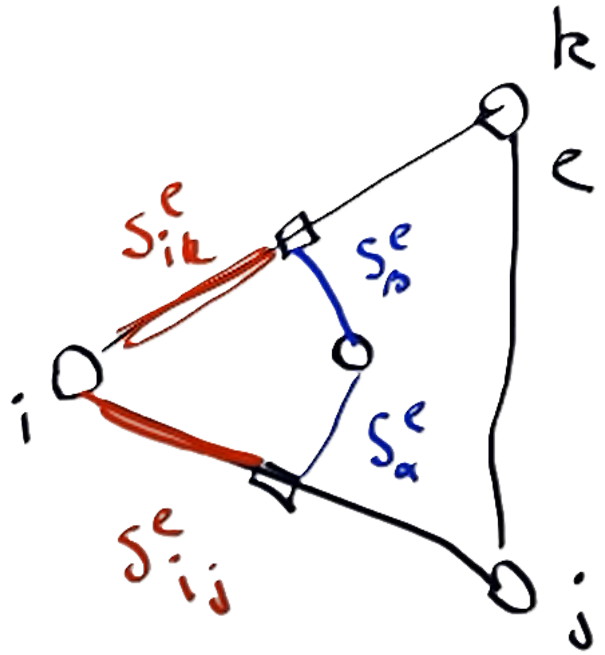
\includegraphics[width=0.2\textwidth]{Images/elem1.png}
  \caption{One of vertex $i$'s neighbouring elements $e$.\label{fig:elem1}}
\end{figure}
%
Therefore we can rewrite the elastic force term as
%
\begin{equation}
  m_i \ddot{\boldsymbol x}_i = \boldsymbol f_{\mathrm{ext},i} + \boldsymbol f_{t, i} + \underbrace{ \sum_e - \boldsymbol P^e \left( \boldsymbol N_{ij}^e \,l_{ij}^e + \boldsymbol N_{ik}^e \,l_{ik}^e \right)  }_{ \boldsymbol f_{\mathrm{ela}, i} },
\end{equation}
%
where $l_{ij}^e = \lVert \boldsymbol S_{ij}^e \rVert$. Notice that $l_{ij}^e$ is only half the length of the edge, since we're only interested in the part of the edge that belongs to the $i$'th control volume.


\subsection*{Step 6: Time integration}
We have a second order system
%
\begin{equation}
  m_i \ddot{\boldsymbol x}_i = \boldsymbol f_{\mathrm{tot},i}, \qquad \dot{\boldsymbol v}_i = \frac{\boldsymbol f_{\mathrm{tot},i}}{m_i}, \qquad \dot{\boldsymbol x}_i = \boldsymbol v_i
\end{equation}
%
We use the FDA to get
%
\begin{equation}
  \boldsymbol v_i^{t + \Delta t} \approx \boldsymbol v_i^t + \frac{\boldsymbol f_{\mathrm{tot}, i}}{m_i} \,\Delta t, \qquad \qquad
  \boldsymbol x_i^{t+ \Delta t} = \boldsymbol x_i^t + \boldsymbol v_i^{t+\Delta t} \,\Delta t.
\end{equation}
%
It is worthy to note, that since $\boldsymbol f_{\mathrm{tot}, i}$ is evaluated at time $t$, the first equation is explicit in time, but since we use $\boldsymbol v_i^{t + \Delta t}$ in the second equation, this is implicit. This is sometimes called first order semi-implicit Euler time integration.

Since we already handled the boundary conditions in the previous steps, we can now solve the linear system for each time step, and get the solution to the dynamic hyperelastic problem.

\section{Final computational method}
\begin{itemize}
  \item[Step 1:] Compute the deformation gradient $\boldsymbol F^e$ for all triangles $e$.
  \item[Step 2:] Compute the strain tensor $\boldsymbol E^e$ for all triangles $e$.
  \item[Step 3:] Compute the second Piola–Kirchhoff stress $\boldsymbol S^e$ for all triangles $e$.
  \item[Step 4:] Compute the first Piola-Kirchhoff stress $\boldsymbol P^e$ for all triangles $e$.
  \item[Step 5:] Compute the elastic forces $\sum_e\boldsymbol f_{\mathrm{ela},i}^e$ for all vertices $i$.
  \item[Step 6:] Compute the total forces $\boldsymbol f_{\mathrm{tot}, i}$ for all vertices $i$.
  \item[Step 7:] Velocity update $\boldsymbol v_i^{t+\Delta t}$ for all vertices $i$.
  \item[Step 8:] Position update $\boldsymbol x_i^{t + \Delta t}$ for all vertices $i$.
  \item[Step 9:] Update time $t \to t + \Delta t$.
  \item[] $\uparrow$$\uparrow$$\uparrow \ \ $ Repeat $\ \ \uparrow$$\uparrow$$\uparrow$
\end{itemize}

The first 4 steps, iterate over the neighbouring triangles  $e$ of all vertices and the next 4 steps, iterate over just the vertices.

\begin{figure}
  \centering
  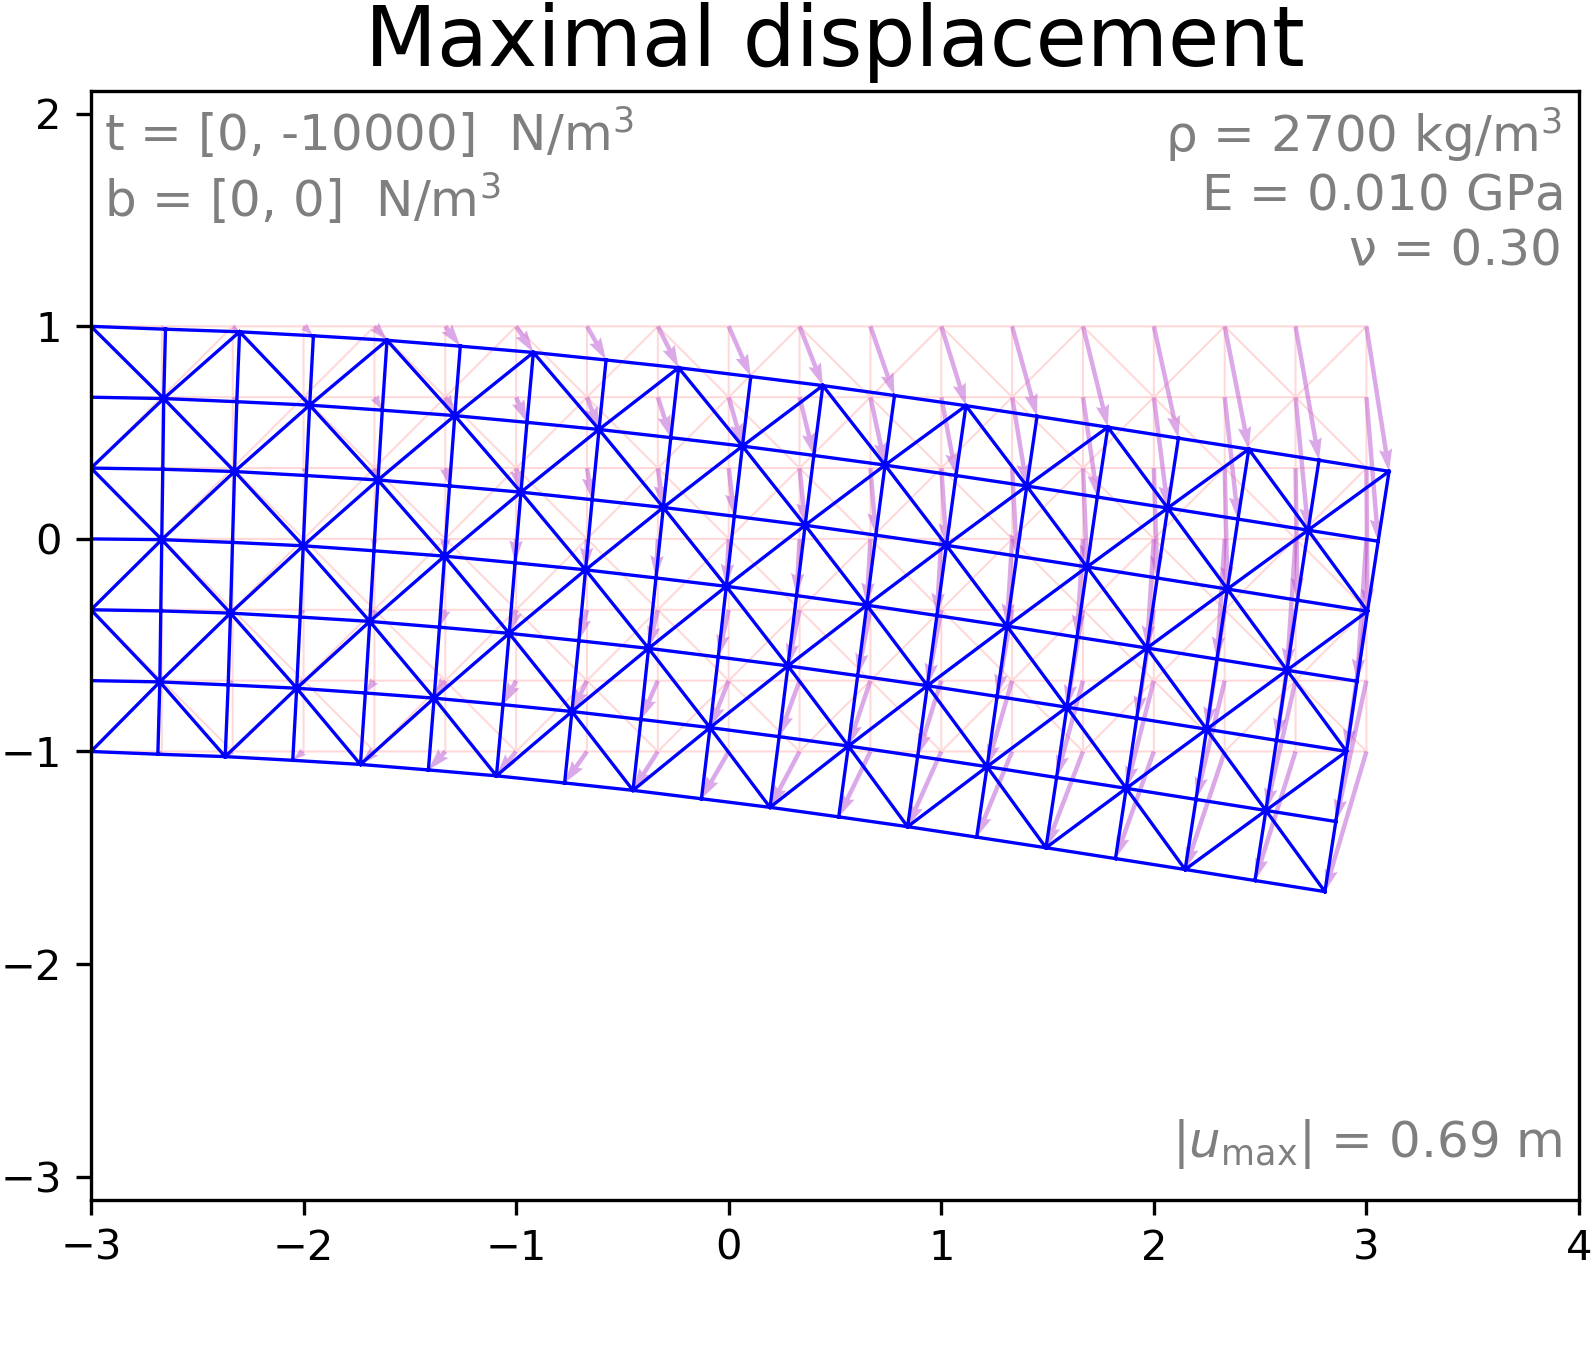
\includegraphics[width=0.3\textwidth]{Images/elastic_cantilever_traction.png}
  \caption{Plot of the maximum deformation for a 10s simulation of the hyperelastic beam with only traction enforced at the right edge vertices. The body force på unit volume $\boldsymbol b$, the material density $\rho$, the material properties $E$ and $\nu$ and the largest deformation $\left\lVert \boldsymbol u_\mathrm{max}  \right\rVert $ are given in the plot.\label{fig:elastic_cantilever_traction}}
\end{figure}

\begin{figure}
  \centering
  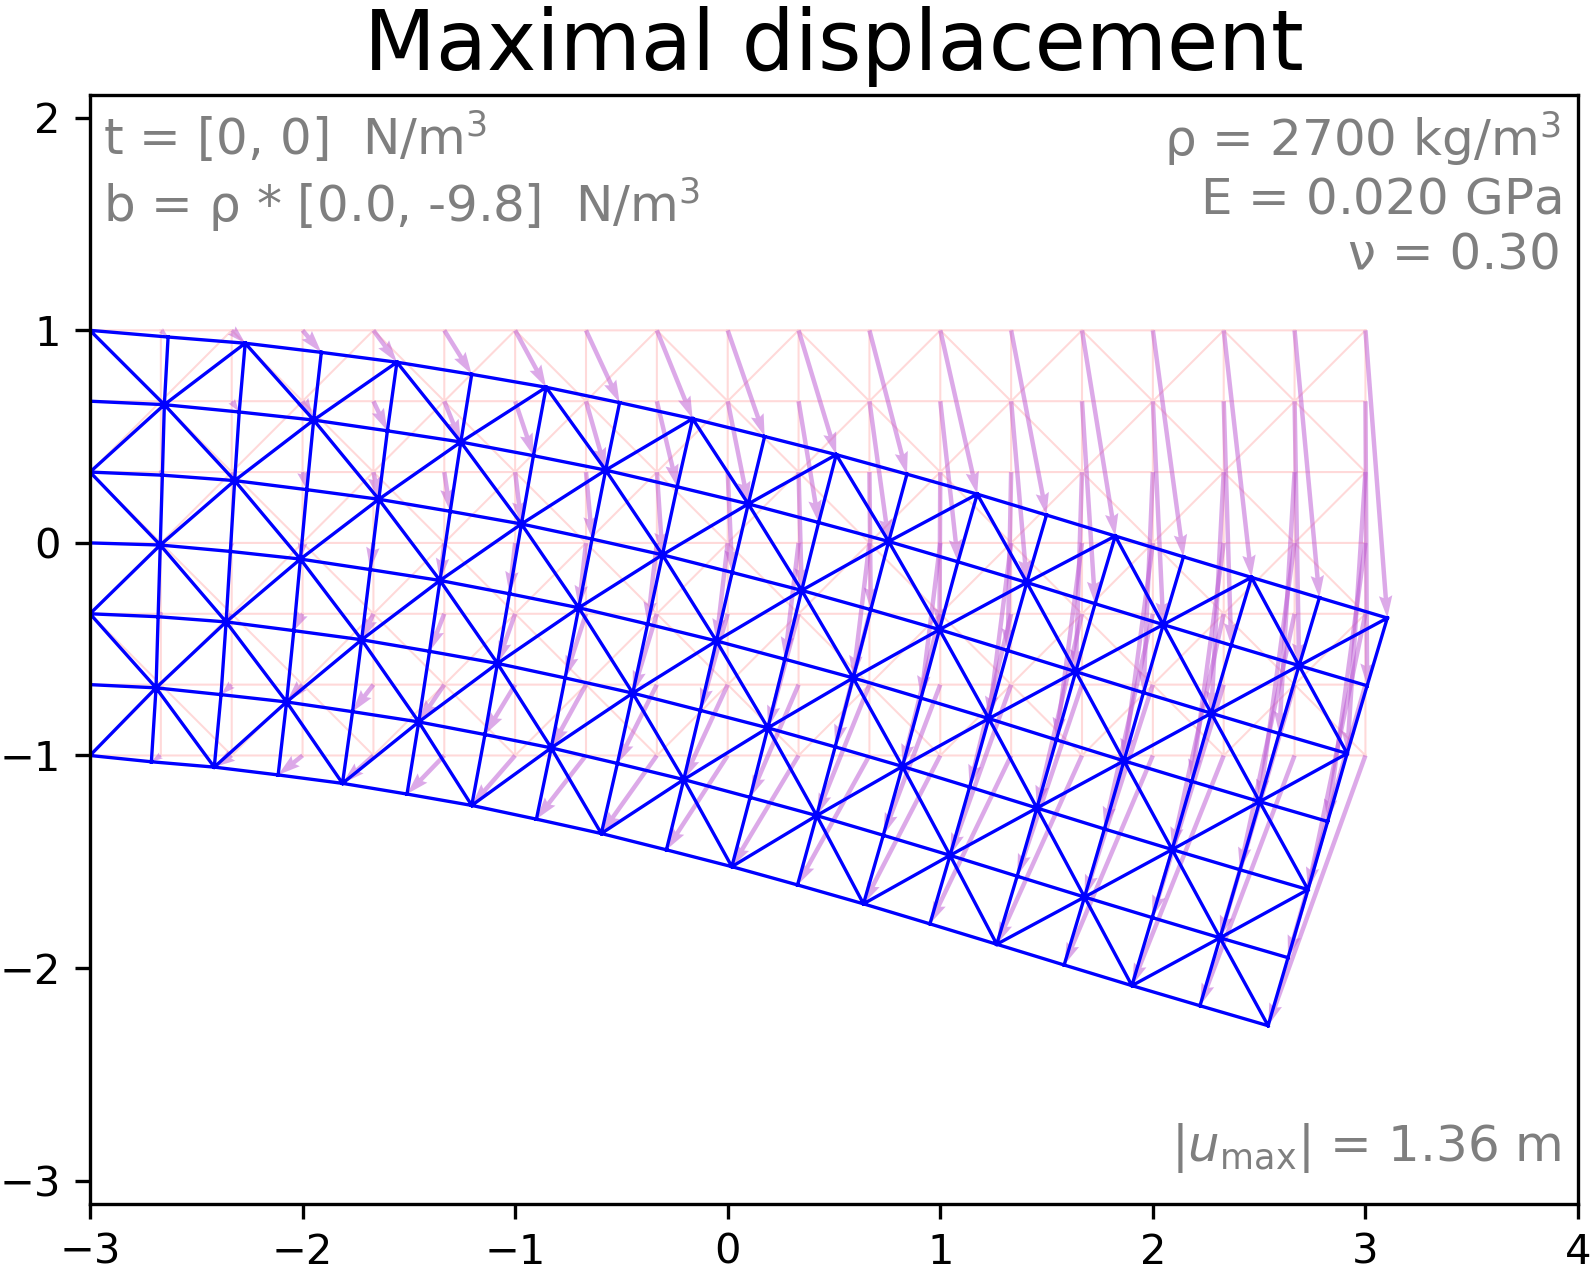
\includegraphics[width=0.3\textwidth]{Images/elastic_cantilever_gravity.png}
  \caption{Plot of the maximum deformation for a 10s simulation of the hyperelastic beam with only gravity. The body force på unit volume $\boldsymbol b$, the material density $\rho$, the material properties $E$ and $\nu$ and the largest deformation $\left\lVert \boldsymbol u_\mathrm{max}  \right\rVert $ are given in the plot.\label{fig:elastic_cantilever_gravity}}
\end{figure}

\end{document}
\endinput
